% =============================================================================
% Any2Ego -- ICLR 2027 submission (rewritten manuscript).
% Compile with pdfLaTeX. Style files (iclr2027_conference.sty/.bst), natbib.sty
% and fancyhdr.sty are already present in this directory.
% The earlier draft is kept untouched in iclr2027_paper.tex.
% =============================================================================
\documentclass{article}
\usepackage{iclr2027_conference,times}

\usepackage{graphicx}
\usepackage{booktabs}
\usepackage{amsmath}
\usepackage{amssymb}
\usepackage{bbm}
\usepackage{natbib}
\usepackage{hyperref}
\usepackage{url}
\usepackage{xcolor}
\usepackage{multirow}
\usepackage{subcaption}
\usepackage{enumitem}
\usepackage{array}
\usepackage{wrapfig}

\newcommand{\PreserveBackslash}[1]{\let\temp=\\#1\let\\=\temp}
\newcolumntype{C}[1]{>{\PreserveBackslash\centering}p{#1}}

\captionsetup{skip=4pt}
\setlength{\textfloatsep}{8pt plus 2pt minus 2pt}
\setlength{\floatsep}{6pt plus 2pt minus 2pt}
\setlength{\intextsep}{6pt plus 2pt minus 2pt}
\setlist{itemsep=1pt,topsep=2pt,parsep=0pt}

% \iclrfinalcopy

\title{Any2Ego: Egocentric Viewpoint Translation\\
Taking Textual Modality as Anchor}

\author{Anonymous authors \\ Paper under double-blind review}

\begin{document}

\maketitle

\begin{abstract}
Egocentric video is the format in which embodied agents see the world and
the format that is hardest to collect, while third-person recordings of the same
activities are abundant, so egocentric viewpoint translation turns a plentiful
resource into a scarce one. Existing methods cast this translation as a direct
cross-view mapping conditioned on a spatial prior such as a hand--object
interaction (HOI) mask, which fixes where the interaction happens and leaves
unconstrained what it looks like from the first person. In this paper, we
introduce \textbf{Any2Ego}, which replaces the direct mapping with translation
through an explicit intermediate modality and takes the \emph{textual modality}
as its anchor. Any2Ego produces both halves of that modality, a predicted HOI
mask and a first-person caption from a converter trained by difference-weighted
distillation and generation-grounded reinforcement, and injects the caption
through HOI-conditioned spatial routing that gates it at every video token. On
held-out Ego-Exo4D clips, the textual anchor reduces FVD from 42.6 to 33.3 over
our reproduced EgoExo-Gen while no component reads a ground-truth egocentric
frame at inference.
\end{abstract}

\section{Introduction}
\label{sec:intro}

Egocentric video is the format in which embodied agents see the world, with the
hands inside the field of view, a viewpoint that moves with the head, and heavy
self-occlusion of the manipulated object~\citep{grauman2024egoexo4d}. However, it
is also the format that is hardest to obtain at scale, because every clip needs a
head-mounted camera on a real wearer, whereas third-person recordings of the same
activities exist in quantity. Egocentric viewpoint translation, which synthesizes
the first-person video of a manipulation task from a third-person observation of
it, therefore turns a plentiful resource into a scarce one. The value of such data
rests entirely on whether the generated video preserves the interaction that the
demonstration shows.

\begin{figure}[t]
\centering
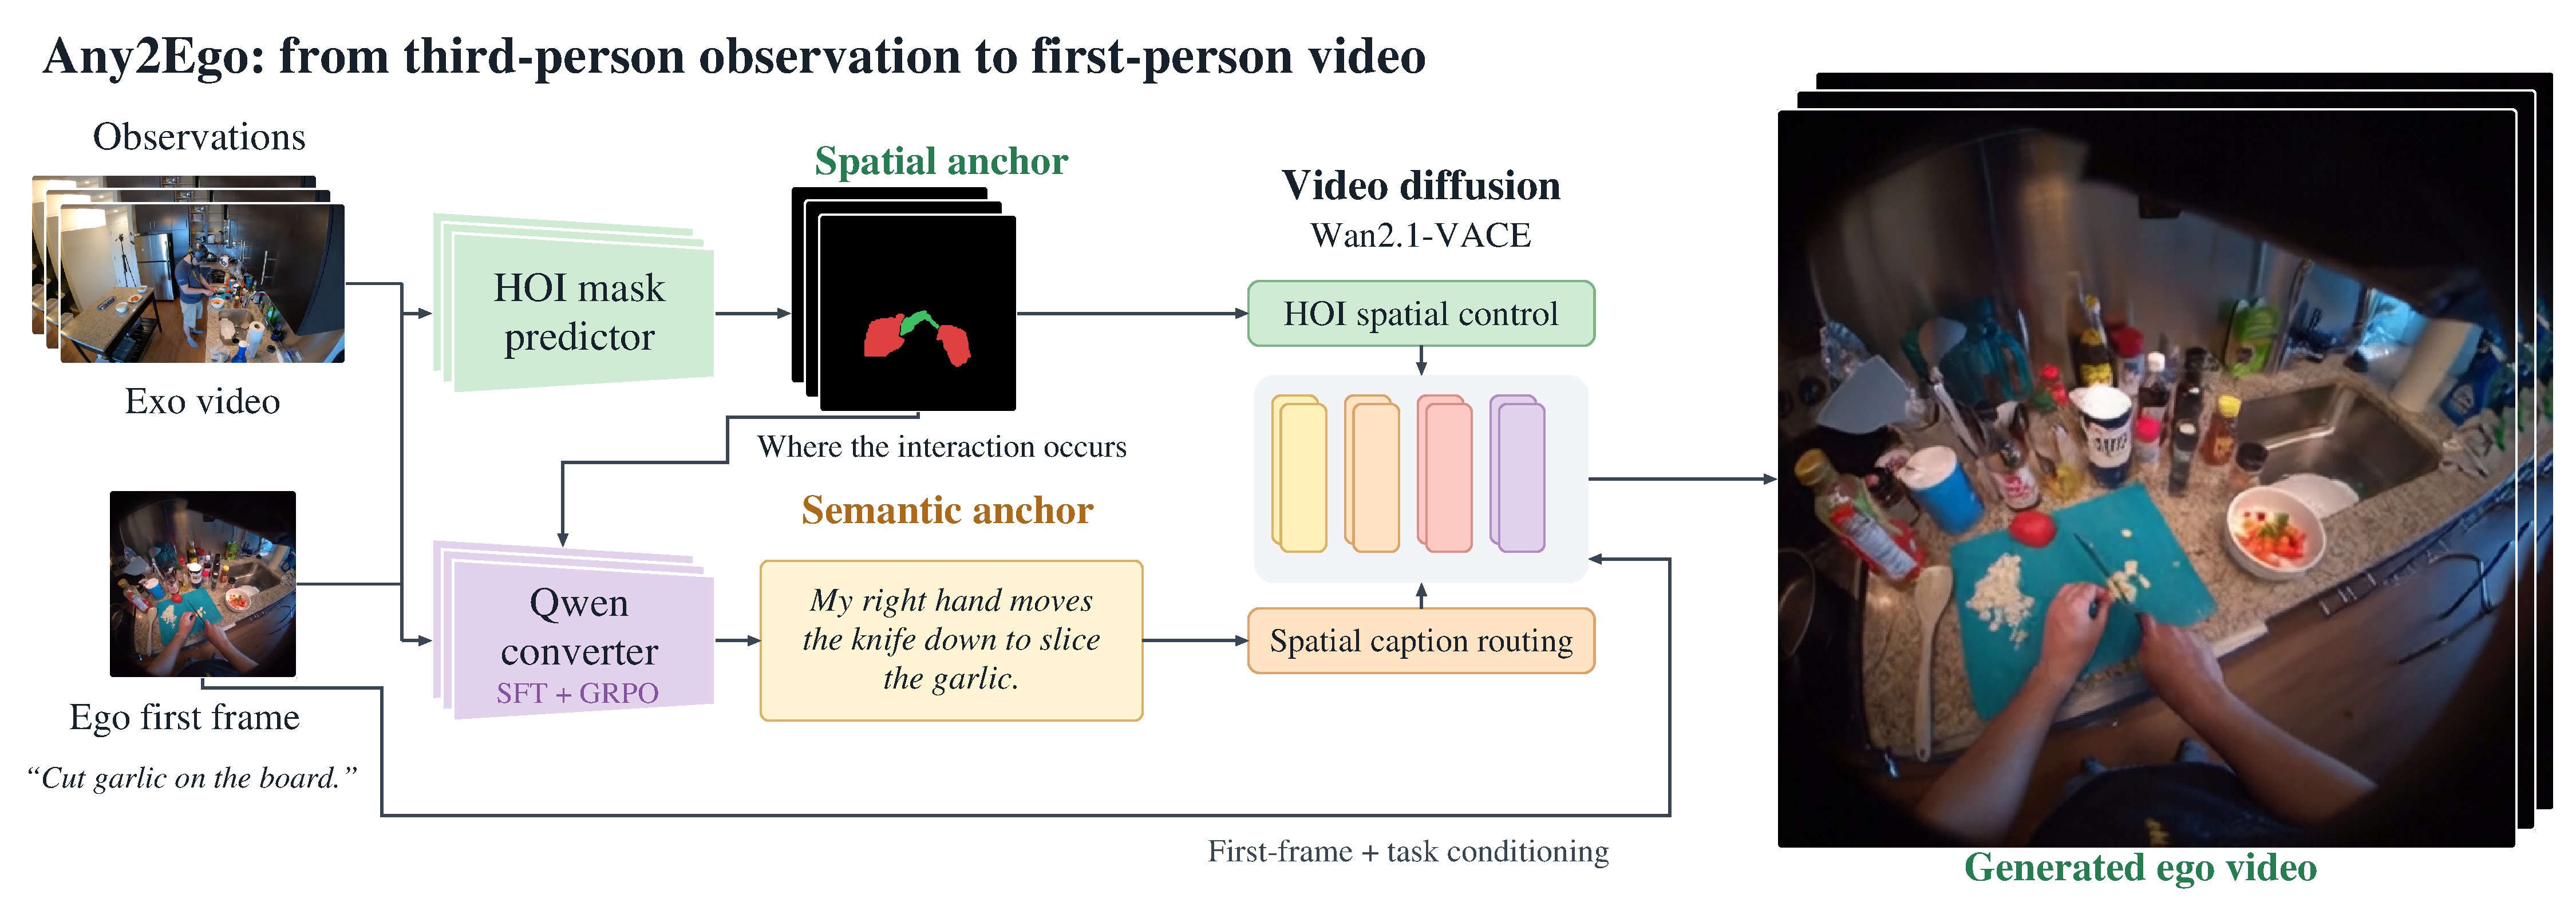
\includegraphics[width=0.94\textwidth]{figs/teaser_overview.pdf}
\caption{Any2Ego turns one hard cross-view mapping into two easier ones by
translating through an explicit intermediate modality, where a produced
spatial anchor states where the interaction happens and a produced textual
anchor states what it looks like from the first person, and HOI-conditioned
spatial routing decides where the textual anchor takes effect.}
\label{fig:teaser}
\end{figure}

This translation is far harder than a change of camera pose. Most of what fills
an egocentric frame is invisible in the exocentric one, because the performer's
body occludes the workspace and the egocentric view is dominated by the hands, so
the two views share no dense pixel correspondence a network could regress. A
direct mapping then asks one model to understand the action, relocate it into the
wearer's body frame, and synthesize first-person appearance in one step, with no
intermediate quantity to supervise or inspect when the output is wrong. A person works in two steps instead,
first resolving where the interaction is, which hand acts on which object and how
they contact, and then resolving what it looks like from the first person, where
the objects fall in the field of view and how the scene appears. A direct mapping
collapses both steps into one.

Existing approaches to egocentric video generation can be broadly categorized
into \emph{spatially conditioned translators} and \emph{general video generators}.
Along the first line, EgoExo-Gen~\citep{xu2025egoexogen} transfers HOI masks
across views and EgoX~\citep{kang2025egox} builds a geometric prior from depth,
point clouds, and camera poses. However, these answer only the first of the two
questions above, since a mask or a depth map specifies neither object appearance,
nor the meaning of a contact, nor how the scene reads from the wearer's eyes. A
second line develops general video backbones such as Stable Video
Diffusion~\citep{blattmann2023svd}, ConsistI2V~\citep{ren2024consisti2v},
Wan~\citep{wan2025}, and VACE~\citep{vace2025}. Although they accept visual and
textual controls, they perform no cross-view conversion of their own and offer no
mechanism deciding where an external semantic condition takes effect. Every explicit intermediate representation proposed so far is
spatial, because geometry is the part of an interaction that transfers across
views by construction, so the second question has never been given a carrier of
its own and remains answered inside the generator weights.

To this end, we introduce \textbf{Any2Ego}, which performs egocentric viewpoint
translation through an explicit intermediate modality and takes the textual
modality as its anchor. A first-person sentence is the natural carrier of the
second question, since it states the interaction in the target viewpoint, it is
discrete and therefore inspectable, and it lands in the text space the video
backbone already consumes. The discreteness of that carrier is what does the work, since the same semantics
passed as continuous vision-language features leaves the video distribution at
the level of the mask condition alone, as Section~\ref{sec:modality} shows. As shown in Figure~\ref{fig:teaser}, Any2Ego
produces both halves of that modality instead of assuming them. Specifically, to
keep the spatial anchor available without an oracle, a cross-view mask predictor
estimates the egocentric HOI-mask sequence. To make the textual anchor carry what
the existing conditions lack, a Qwen3-VL-8B converter is trained by
difference-weighted caption distillation, which concentrates the gradient on
content that a baseline caption from the same deployable inputs fails to express,
and then by generation-grounded reinforcement learning, whose reward measures how
well a rendered preview agrees with the newly added sentences. To apply the anchor only where its content is
relevant, we propose HOI-conditioned spatial routing, which reuses the dense
features of the control branch to gate every video token. Any2Ego thereby turns
one hard cross-view mapping into two easier ones that are trained and inspected
separately.

Experiments on held-out Ego-Exo4D cooking clips show that the textual anchor
improves every metric over EgoExo-Gen, reducing FVD from 42.6 to 37.8 under a
global gate and to 33.3 under spatial routing, and that our converter surpasses the strongest off-the-shelf model on judged
first-person faithfulness by 0.915 composite. Notably, every reported number
comes from the deployed pipeline, since no component reads a ground-truth
egocentric frame at inference.
In summary, our key contributions are three-fold.
\begin{itemize}[leftmargin=1em, itemsep=-1ex, topsep=0ex]
    \item \textbf{Textual Anchor:} To the best of our knowledge, Any2Ego is
    the first exo-to-ego framework whose intermediate modality is \emph{not
    spatial}, and the discreteness of that modality is what carries the gain,
    since the same semantics passed as continuous vision-language features gives
    no distributional improvement under an identical injection gate.
    \item \textbf{Anchor Production and Routing:} We propose
    difference-weighted caption distillation with generation-grounded
    reinforcement learning to produce the textual anchor from deployable inputs,
    and we derive in closed form how much caption signal a single per-block gate
    loses, a quantity that grows with the response energy the branch spends where
    the caption is irrelevant and that motivates HOI-conditioned spatial routing.
    \item \textbf{Strong Performance:} On held-out Ego-Exo4D clips, Any2Ego
    reduces FVD from 42.6 to 33.3 over EgoExo-Gen and reaches a residual motion
    correlation of 0.647 against 0.561 for it and 0.233 for the strongest
    image-to-video baseline.
\end{itemize}

\section{Related Work}
\label{sec:related}

\textbf{Egocentric Video Generation.}\quad Existing methods for generating
egocentric video from third-person observations differ mainly in the
intermediate representation they make explicit.
EgoExo-Gen~\citep{xu2025egoexogen} predicts egocentric HOI masks through
cross-view memory attention and conditions a diffusion backbone on them, which
transfers the layout of hands and manipulated objects across views.
EgoX~\citep{kang2025egox} instead reconstructs a geometric egocentric prior
from depth, point clouds, and camera poses, and renders it as a conditioning
signal. Both confirm that an explicit intermediate condition beats an unconstrained
mapping. However, both representations are purely spatial, so object appearance,
contact semantics, and the first-person reading of the scene stay unspecified.

\textbf{Controllable Video Diffusion.}\quad A parallel line of work develops the
backbones on which such translators are built. Stable Video
Diffusion~\citep{blattmann2023svd} and ConsistI2V~\citep{ren2024consisti2v}
animate a single image, CogVideoX~\citep{yang2024cogvideox} and
LTX-Video~\citep{hacohen2025ltxvideo} scale text-conditioned latent diffusion, and
Wan~\citep{wan2025} with VACE~\citep{vace2025} adds a control branch for masks and
reference frames. Overall, no prior method in either line supplies an intermediate condition that
is not spatial, and none decides where a semantic condition should act inside the
frame. Unlike
previous approaches that condition generation on a spatial prior alone, Any2Ego
adopts a more deliberate design by producing a first-person textual anchor with
a trained converter and routing it through HOI-conditioned per-token gates, so
the second step of human cross-view reasoning becomes explicit and trainable.

\section{Any2Ego}
\label{sec:method}

In this paper, we introduce Any2Ego, a framework that performs egocentric
viewpoint translation through an explicit intermediate modality anchored on
text. To relieve the generator of the two reasoning steps that a direct mapping
collapses, Any2Ego separates that modality into a spatial anchor and a textual
anchor, and produces both with trained modules so no condition is an
oracle at inference. The framework, the two anchor producers, the
routing module, and the freeze-frame calibration that makes the reported metrics
interpretable are introduced as follows.

\subsection{Framework}
\label{sec:framework}

Let $X=\{X_t\}_{t=0}^{T-1}$ denote the exocentric video, $S$ its HOI masks,
$I_0$ the egocentric first frame, $M_0$ its mask, and $n$ the task narration.
Any2Ego consists of a cross-view mask predictor $f_{\mathrm{seg}}$, a caption
converter $f_{\mathrm{cap}}$, and a video generator $f_{\mathrm{gen}}$ built on
Wan2.1-VACE-1.3B~\citep{wan2025,vace2025}.
The three form a feed-forward pipeline, where the predictor estimates the
egocentric interaction geometry, the converter describes it in first-person
language, and the generator synthesizes the egocentric video under both
conditions,
\begin{equation}
\widehat{M} = f_{\mathrm{seg}}(X,S,I_0,M_0),\qquad
c \sim f_{\mathrm{cap}}(\cdot\mid X,I_0,\widehat{M},n),\qquad
\widehat{Y} = f_{\mathrm{gen}}(I_0,\widehat{M},n,c),
\label{eq:pipeline}
\end{equation}
where $\widehat{M}$ is the predicted HOI-mask sequence, $c$ the first-person
caption, and $\widehat{Y}$ the generated video, as illustrated in
Figure~\ref{fig:pipeline}. The caption is conditioned on
the predicted mask and never on a ground-truth egocentric frame, so every
quantity in Eq.~\ref{eq:pipeline} is available at deployment.

\subsection{Interaction-Grounded Spatial Anchor}
\label{sec:seg}

To make the interaction geometry available at deployment without reading any
ground-truth egocentric mask, we implement $f_{\mathrm{seg}}$ following the
cross-view memory-attention formulation of EgoExo-Gen~\citep{xu2025egoexogen}. A
shared ResNet-18
encoder embeds both views, a mask-conditioned value encoder fuses the egocentric
first-frame condition, cross-view memory attention lets each exocentric query
retrieve the matching egocentric appearance, and a decoder predicts background,
hand, and object labels. We train it with class-weighted cross-entropy plus a soft Dice term on the
two foreground classes, which optimizes foreground overlap,
\begin{equation}
\mathcal{L}_{\mathrm{seg}} = \mathcal{L}_{\mathrm{CE}}
+ \mathcal{L}_{\mathrm{Dice}},
\label{eq:seg}
\end{equation}
where $\mathcal{L}_{\mathrm{CE}}$ uses weights $1{:}5{:}5$ over background,
hand, and object. The predictor exports masks in the generator's input format, which makes the
spatial anchor of Eq.~\ref{eq:pipeline} a predicted quantity in every
experiment.

\subsection{First-Person Textual Anchor}
\label{sec:cap}

To supply the semantics that a mask cannot express, $f_{\mathrm{cap}}$
converts the visual conditions into a structured first-person caption with six
fields, namely \texttt{HANDS}, \texttt{OBJECT}, \texttt{CONTACT},
\texttt{SCENE}, \texttt{MOTION}, and \texttt{LIGHTING}. We build it from Qwen3-VL-8B-Instruct,
freeze the visual encoder and the aligner, and adapt the language model with
rank-16 LoRA. Its input $u=(X,I_0,\widehat{M},n,\iota)$ collects the exocentric
video, the egocentric first frame, the predicted masks, the narration, and a
viewpoint instruction $\iota$. The difficulty is that a capable vision-language
model already describes much of what the masks and the first frame make visible,
so imitating a teacher caption directly spends most of its gradient on content the
generator already sees, which the two training stages below address.

\textbf{Difference-weighted Caption Distillation.}\quad To concentrate supervision on what
the existing conditions fail to carry, we compare each teacher sentence against
what the converter itself would say from the deployable inputs alone. Teacher
captions $c^\star$ come offline from a 27B vision-language model that reads the
paired egocentric footage, and a baseline caption $b$ is generated from $u$ alone.
Aligning the two separates new from redundant content, and we set the token weight
$w_j$ to $2.5$, $0.3$, and $1.0$ for new, redundant, and partially overlapping
content. For a target of length $L$, the
weighted objective is
\begin{equation}
\mathcal{L}_{\mathrm{cap}}(\theta) = -\mathbb{E}_{(u,c^\star)}\left[
\frac{1}{L}\sum_{j=1}^{L} w_j \log \pi_\theta\!\left(c^\star_j \mid u,
c^\star_{<j}\right)\right],
\label{eq:sft}
\end{equation}
where $\pi_\theta$ is the converter policy with trainable LoRA parameters
$\theta$. Reweighting leaves the target text unchanged and only redistributes gradient
mass, so the converter still learns the full six-field structure while being
pushed toward content absent from $b$.

\textbf{Generation-grounded Caption Reinforcement.}\quad To align the
converter with what the generator can actually use, we continue from the
distilled checkpoint with GRPO~\citep{shao2024grpo} and define a reward on
rendered video instead of on text similarity. For each input the rollout policy samples $G=8$
candidates, a frozen generator renders a preview $\widehat{Y}_i$ for candidate
$c_i$, and the preview is cropped to the union bounding box of the HOI masks so
the reward is measured where the interaction is. Let $\mathcal{S}_i$ be the new
sentences of $c_i$, $C_M$ the crop operator, and $e_I, e_T$ unit-normalized
CLIP~\citep{radford2021clip} embeddings. With $F$ preview frames, the reward is
\begin{equation}
r_i = \frac{1}{F|\mathcal{S}_i|}\sum_{t=1}^{F}\sum_{s\in\mathcal{S}_i}
e_I\!\left(C_M(\widehat{Y}_{i,t})\right)^{\!\top} e_T(s),
\label{eq:reward}
\end{equation}
where the candidate is scored on its full text when no new sentence is
identified. We optimize Eq.~\ref{eq:reward} with the clipped GRPO objective under
group-normalized advantages and a KL term to a fixed reference policy, updating
only the converter LoRA while the generator and CLIP stay frozen.
Appendix~\ref{app:impl} details both stages, which
Figure~\ref{fig:qwen} summarizes.

\begin{figure}[t]
\centering
\begin{subfigure}[b]{\textwidth}
\centering
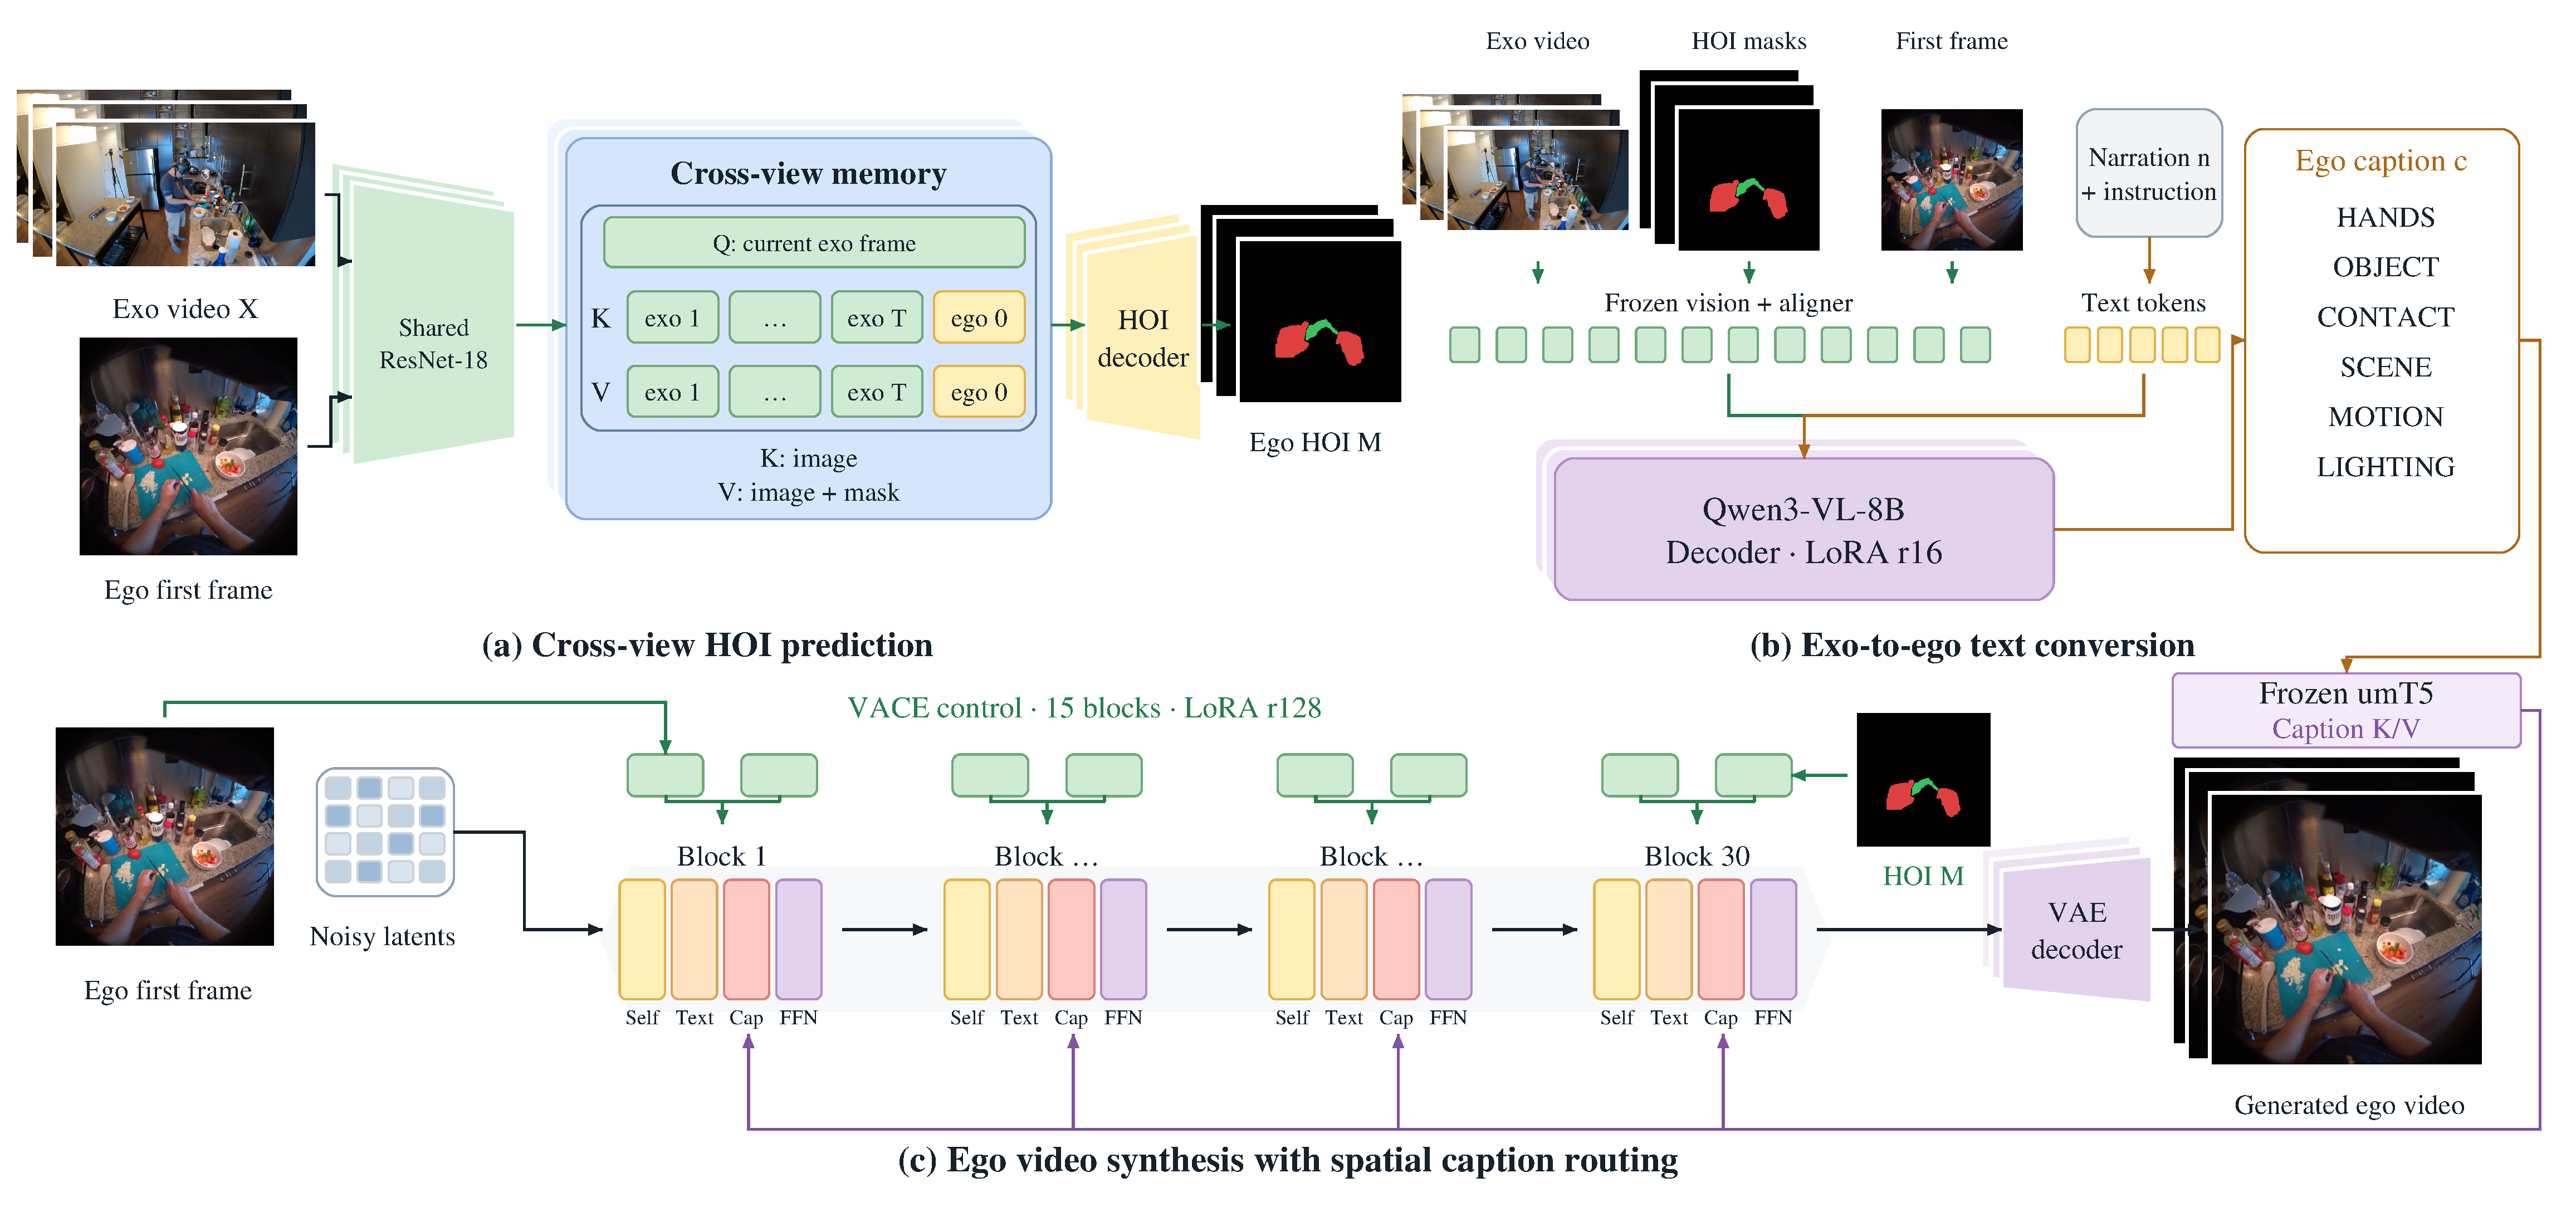
\includegraphics[width=\textwidth]{figs/architecture_illustration.pdf}
\caption{Any2Ego pipeline.}
\label{fig:pipeline}
\end{subfigure}

\begin{subfigure}[b]{\textwidth}
\centering
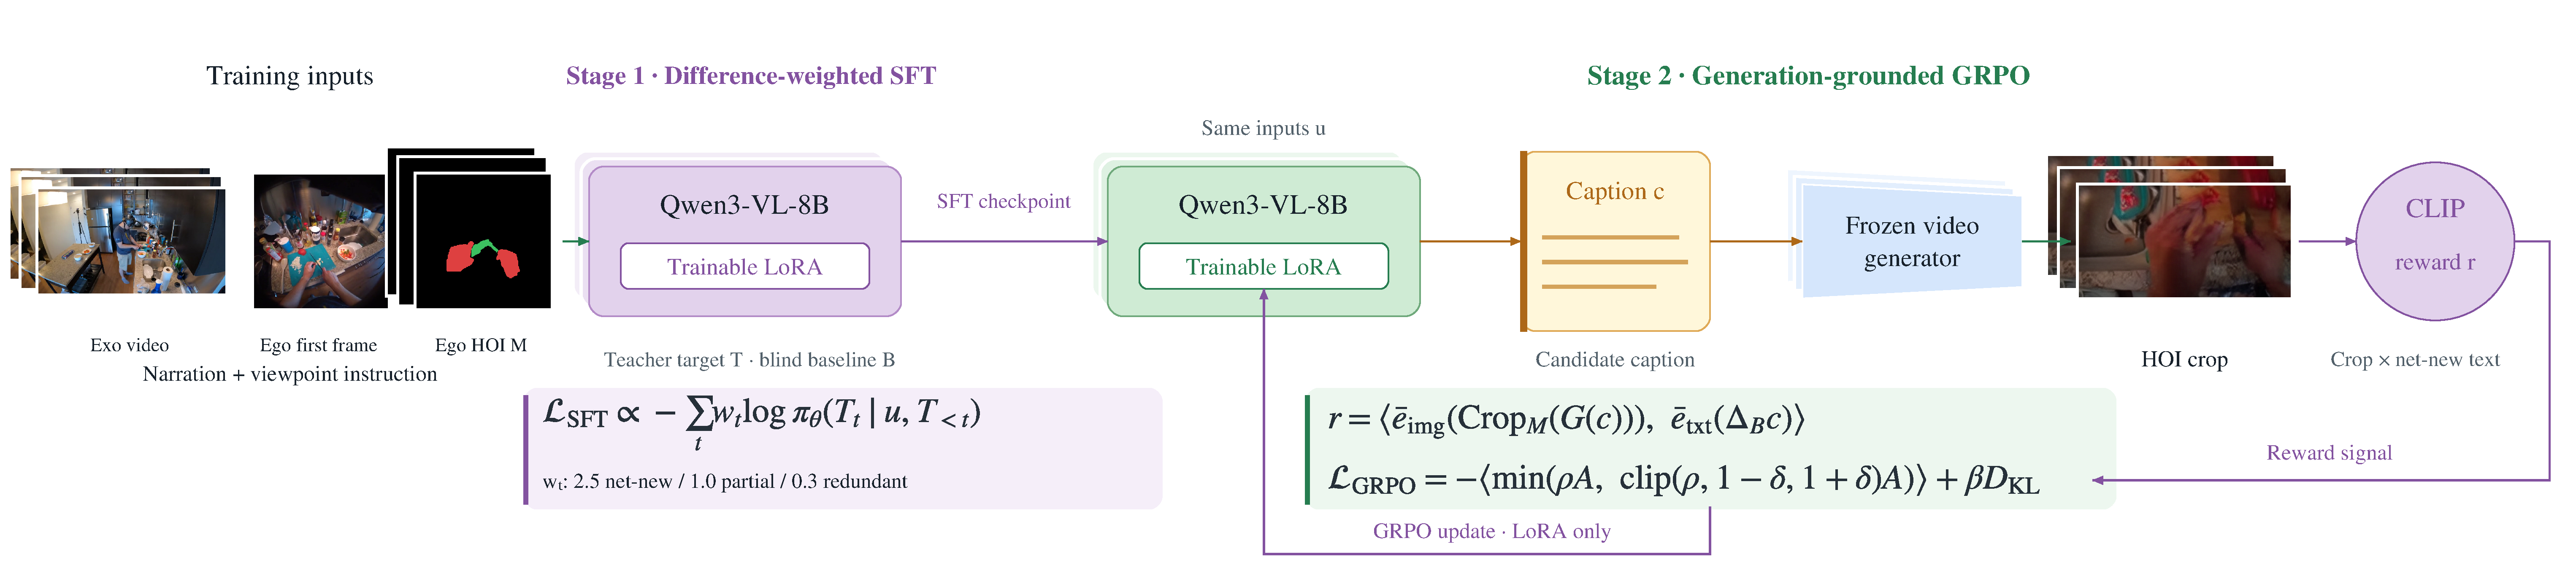
\includegraphics[width=\textwidth]{figs/qwen_architecture.pdf}
\caption{Training of the cross-view caption converter.}
\label{fig:qwen}
\end{subfigure}
\caption{(a) Any2Ego produces the spatial anchor with a cross-view mask predictor
and the textual anchor with a distilled and reinforcement-refined converter, then
combines them in a mask-conditioned backbone whose caption branch is gated per
video token by the dense spatial features of the control branch.
(b) Difference-weighted distillation concentrates the gradient on caption content
that the deployable inputs do not already express, and generation-grounded
reinforcement scores each candidate by how well a rendered preview agrees with its
newly added sentences inside the interaction region.}
\end{figure}

\subsection{HOI-Conditioned Spatial Routing}
\label{sec:routing}

To let the textual anchor act where its content applies, we design the injection
path so its strength varies across the frame. The predicted masks $\widehat{M}$
enter Wan2.1-VACE through its 15-block control branch, while $I_0$ provides the
image condition and $n$ uses the native text path. The caption $c$ is encoded by a
frozen umT5 into $E_c$, and we attach a caption cross-attention branch to each of
the 30 main blocks, reusing the video queries $Q^{(\ell)}$ and learning caption
projections,
\begin{equation}
A_c^{(\ell)} = \operatorname{softmax}\!\left(
\frac{Q^{(\ell)}\left(E_c W_{K,c}^{(\ell)}\right)^{\!\top}}{\sqrt{d}}\right)
E_c W_{V,c}^{(\ell)},
\label{eq:capattn}
\end{equation}
where $d$ is the head dimension and $W_{K,c}^{(\ell)}$, $W_{V,c}^{(\ell)}$ are
the only new projections in the block. The caption response is then scaled and
added to the native attention before the frozen output projection,
\begin{equation}
O_i^{(\ell)} = W_O^{(\ell)}\!\left[A_{\mathrm{native},i}^{(\ell)}
+ g^{(\ell)} s_i^{(\ell)} A_{c,i}^{(\ell)}\right],\qquad
s_i^{(\ell)} = \sigma\!\left(\left(w^{(\ell)}\right)^{\!\top}
\operatorname{sg}(m_i) + b^{(\ell)}\right),
\label{eq:route}
\end{equation}
where $m_i$ is the pre-block HOI feature of the control branch aligned with video
token $i$, $\operatorname{sg}$ stops gradients, and $\sigma$ is the sigmoid.
Setting $s_i^{(\ell)}\!=\!1$ recovers a global gate and $g^{(\ell)}\!=\!0$ removes
the caption. We initialize $g^{(\ell)}=0.1$ and $w^{(\ell)}=b^{(\ell)}=0$, so
routing starts from the neutral factor $0.5$ and cannot destabilize the trained
spatial branch.

\textbf{Dilution of a Global Gate.}\quad To explain why the per-token factor
matters, we analyze one block at one denoising step with its attention
responses held fixed. A global gate already produces token-dependent responses,
because the video queries in Eq.~\ref{eq:capattn} differ across locations, and
its limitation is the shared \emph{scaling} of those responses. Writing
$a_i=W_O A_{c,i}$ for the projected caption response at token $i$ and $r_i$ for
the local correction the mask-conditioned representation still needs, the two
designs minimize
\begin{equation}
\mathcal{E}_{\mathrm{global}}(g)=\sum_i\left\|r_i-g a_i\right\|_2^2,
\qquad
\mathcal{E}_{\mathrm{route}}(g,s)=\sum_i\left\|r_i-g s_i a_i\right\|_2^2 .
\label{eq:error}
\end{equation}
Consider a caption relevant on a token set $\mathcal{F}$, so $r_i=\kappa a_i$ for
$i\in\mathcal{F}$ with $\kappa>0$ and $r_i=0$ elsewhere. Writing
$E_{\mathcal{F}}=\sum_{i\in\mathcal{F}}\|a_i\|_2^2$ and
$E_{\overline{\mathcal{F}}}=\sum_{i\notin\mathcal{F}}\|a_i\|_2^2$ for the
response energies inside and outside that set, the optimal global gate and its
residual are
\begin{equation}
g^*=\kappa\,\frac{E_{\mathcal{F}}}
{E_{\mathcal{F}}+E_{\overline{\mathcal{F}}}},\qquad
\mathcal{E}_{\mathrm{global}}(g^*)=\kappa^2\,
\frac{E_{\mathcal{F}}E_{\overline{\mathcal{F}}}}
{E_{\mathcal{F}}+E_{\overline{\mathcal{F}}}},
\label{eq:dilution}
\end{equation}
where the residual vanishes only when one of the two energies vanishes. A single
scalar must therefore trade the tokens that need a correction against those
producing the same response without needing one, and the loss grows with the
energy the branch spends outside $\mathcal{F}$. A spatial factor approaching $1$
on $\mathcal{F}$ and $0$ elsewhere removes this residual at $g=\kappa$, and the
implemented sigmoid gate approximates such selectivity from HOI features. The
dilution is a property of any single-gate semantic branch, so it becomes visible
only once such a branch exists, and it predicts the ordering that
Section~\ref{sec:effect-routing} measures. Notably, relevance is caption-dependent and need not coincide with the hand and
object foreground, because the caption also describes scene and lighting.

\textbf{Two-stage Generator Training.}\quad To keep any comparison between
injection designs attributable to the injection itself, stage one fits rank-128
LoRA on the VACE control branch with the backbone frozen, which reproduces
EgoExo-Gen's mask conditioning and is shared by all variants, and stage two
freezes that base and trains only the caption projections and gates under caption
dropout. Both stages use the flow-matching objective of the backbone,
\begin{equation}
\mathcal{L}_{\mathrm{gen}}(\psi)=\mathbb{E}_{z,\epsilon_z,\tau}\left[
\omega(\tau)\operatorname{MSE}\!\left(P_{+}v_\psi(z_\tau,\tau;\mathcal{C}),\,
P_{+}(\epsilon_z-z)\right)\right],
\label{eq:flow}
\end{equation}
where $z_\tau=(1-\tau)z+\tau\epsilon_z$, $z$ is the encoded egocentric video,
$\epsilon_z$ is Gaussian noise, $\omega(\tau)$ the scheduler weight, $P_{+}$
excludes the fixed first latent frame, and $\mathcal{C}$ collects
$(I_0,\widehat{M},n)$ in stage one and $(I_0,\widehat{M},n,c)$ in stage two.
Because stage two changes only the caption path, the reproduced baseline, the
global gate, and the full model differ in exactly one design decision.

\subsection{Freeze-Frame Calibration}
\label{sec:freeze}

To compare the injection designs above we need a metric that responds to
generated motion, and on short horizons the common frame-level metrics do
not. An egocentric clip of roughly $1.6$ seconds retains much of the appearance of its
given first frame, so a model earns frame-level credit for holding that frame in
place. We make this measurable with a no-model control that repeats the given
frame at all 13 positions, which has zero generated motion and therefore sets the
score a method must exceed before its frame-level numbers carry information,
\begin{equation}
\widehat{Y}^{\mathrm{freeze}}_t = I_0, \qquad t=0,\dots,12 .
\label{eq:freeze}
\end{equation}
This control reaches $0.601$ SSIM at $21.88$\,dB PSNR on our evaluation pool,
which already exceeds all six open-source generators we evaluate on both metrics,
while its FVD is $357.2$ and its residual correlation with the true motion is
zero by construction. We therefore report FVD as the primary metric, read SSIM and PSNR against the
calibration value, and add the residual-frame diagnostics of
Section~\ref{sec:residual}. It costs one frame copy and applies to any short-horizon
egocentric benchmark, so we report it alongside every method in our tables.

\section{Experiments}
\label{sec:exp}

\subsection{Dataset and Metrics}
\label{sec:data}

\textbf{Ego-Exo4D.}\quad We conduct experiments on the cooking activities of
Ego-Exo4D~\citep{grauman2024egoexo4d}, which provides time-synchronized
exocentric and egocentric recordings of the same task. The generator is trained
on 34{,}242 annotated clips, the converter on 32{,}562, and the mask predictor on
all 108{,}338. For evaluation we randomly sample a pool of $N{=}1{,}000$ clips
whose source takes are disjoint from every training split, and fix this
split for all comparisons. The pool spans 281 takes, 47 settings, 13 tasks,
and 10 collecting institutions. The dataset, annotation, conditioning inputs, and split
construction all follow EgoExo-Gen~\citep{xu2025egoexogen}, so the whole setting
is aligned with prior work and every method in our tables is scored under it.

\textbf{Metrics.}\quad We report FVD, SSIM, PSNR, and LPIPS under the reading of
Section~\ref{sec:freeze}. For caption quality, Qwen3.5-27B scores each caption
against 13 ground-truth egocentric frames on six semantic fields and on overall
faithfulness from 1 to 5, with a composite score that penalizes
recording-equipment mentions and grammar failures.

\subsection{Experimental Setup}
\label{sec:setup}

We build Any2Ego on Wan2.1-VACE-1.3B~\citep{wan2025,vace2025} as the video
backbone and Qwen3-VL-8B-Instruct as the converter, with a frozen umT5 text
encoder and a ResNet-18 mask predictor. We use ms-swift for difference-weighted
distillation and its GRPO trainer with colocated vLLM rollout for the
reinforcement stage, on the Ego-Exo4D cooking splits of
Section~\ref{sec:data}. Our models generate 13-frame clips at
$480\times480$ with 50 denoising steps and a fixed seed, each baseline keeps the
sampler setting of its release, and every metric is computed under one shared
frame-loading pipeline defined in Appendix~\ref{app:eval}. All training and
inference run on NVIDIA A800 GPUs.

\subsection{Main Results}
\label{sec:main}

\textbf{Capability on Cross-view Semantic Conversion.}\quad We first evaluate
$f_{\mathrm{cap}}$ on the $N{=}1{,}000$ pool to assess its \emph{first-person
conversion capability}, where each caption is judged against real egocentric
frames the converter never sees, against off-the-shelf vision-language models from
8B to 235B parameters under identical inputs. As shown in Table~\ref{tab:caption}, our 8B converter attains the
highest composite score of $4.043$ and leads every off-the-shelf model we
evaluate, including one nearly thirty times larger and its own untrained
backbone. More importantly, the two stages act differently, as distillation
establishes the six-field first-person form while generation-grounded
reinforcement raises faithfulness further by favoring content the generator can
render.
Overall, the judged faithfulness of our converter shows that the textual anchor
can be produced at deployment quality from exocentric inputs alone.

\begin{table}[t]
\centering\small
\caption{Our 8B converter produces more faithful first-person descriptions than
off-the-shelf models up to 235B parameters. Label-mean averages the six field
scores, Comp.\ subtracts penalties for recording-equipment mentions (Rule-0)
and grammar failures from Overall, and Gram.\ is the judged pass rate. Best
values are in \textbf{bold}.}
\label{tab:caption}
\begin{tabular}{llC{1.25cm}C{1.3cm}C{1.55cm}C{1.2cm}C{1.2cm}}
\toprule
\textbf{Caption source} & \textbf{Params} & \textbf{Comp.}\,$\uparrow$ & \textbf{Overall}\,$\uparrow$ & \textbf{Label-mean}\,$\uparrow$ & \textbf{Rule-0}\,$\downarrow$ & \textbf{Gram.}\,$\uparrow$ \\
\midrule
\textbf{Any2Ego converter} & 8B & \textbf{4.043} & \textbf{4.051} & \textbf{4.281} & 0.0\% & 97.5\% \\
\textbf{$\;\;$w/o reinforcement} & 8B & 3.689 & 3.790 & 4.160 & 0.6\% & 68.2\% \\
\midrule
Qwen3-VL-32B & 32B & 3.128 & 3.131 & 3.529 & 0.0\% & 99.1\% \\
Qwen3-VL-235B & 235B & 3.079 & 3.079 & 3.430 & 0.0\% & \textbf{99.9\%} \\
Qwen3.5-9B & 9B & 3.003 & 3.004 & 3.354 & 0.0\% & 99.8\% \\
Qwen3-VL-8B & 8B & 2.829 & 2.831 & 3.164 & 0.0\% & 99.3\% \\
\bottomrule
\end{tabular}
\end{table}
\begin{table}[t]
\centering\small
\caption{Any2Ego leads every open-source generator and EgoExo-Gen, which we
reproduce on the same backbone, on all four metrics. Frame-level metrics saturate
on short horizons, since the freeze-frame calibration outscores all six
open-source generators on SSIM and PSNR while ranking near the bottom on FVD.
Sees exo indicates whether a model observes the third-person video. Best values
are in \textbf{bold}.}
\label{tab:main}
\begin{tabular}{lcC{1.35cm}C{1.35cm}C{1.35cm}C{1.35cm}}
\toprule
\textbf{Method} & \textbf{Sees exo} & \textbf{SSIM}\,$\uparrow$ & \textbf{PSNR}\,$\uparrow$ & \textbf{LPIPS}\,$\downarrow$ & \textbf{FVD}\,$\downarrow$ \\
\midrule
Freeze first frame (no model) & no & 0.601 & 21.88 & & 357.2 \\
\midrule
Wan2.1-VACE-1.3B & yes & 0.178 & 10.14 & 0.711 & 1118.7 \\
Wan2.1-Fun-1.3B-Control & yes & 0.368 & 12.30 & 0.844 & 2361.1 \\
Stable Video Diffusion & no & 0.438 & 16.10 & 0.386 & 177.0 \\
Wan2.2-TI2V-5B & no & 0.553 & 20.74 & 0.225 & 127.6 \\
LTX-Video & no & 0.574 & 20.85 & 0.210 & 121.6 \\
CogVideoX-5B-I2V & no & 0.578 & 21.09 & 0.211 & 148.3 \\
EgoExo-Gen (reproduced) & yes & 0.608 & 21.06 & 0.194 & 42.6 \\
\midrule
\textbf{Any2Ego (ours)} & yes & \textbf{0.660} & \textbf{22.28} & \textbf{0.144} & \textbf{33.3} \\
\bottomrule
\end{tabular}
\end{table}

\textbf{Capability on Egocentric Viewpoint Translation.}\quad We then evaluate the full
pipeline to assess its \emph{cross-view translation capability}, where each model
receives its native conditioning inputs and must produce the 13 frames of the
real egocentric continuation. We compare Any2Ego with video-to-video generators that
receive the raw exocentric video, with image-to-video generators that receive the
first frame and the task prompt, each run from its released checkpoint, and with
the freeze-frame calibration. Since EgoExo-Gen~\citep{xu2025egoexogen} is reproduced on the
same backbone, the comparison against it isolates what the textual anchor adds.
As shown in Table~\ref{tab:main}, Any2Ego leads on all four metrics and reaches
$33.3$ FVD, while EgoExo-Gen, the strongest prior method here, already separates
itself from every open-source generator. More importantly, the freeze-frame row
shows why the frame-level columns must be read with care, since a video with no
generated motion outscores all six open-source generators on SSIM and PSNR while
placing near the bottom on FVD. Overall, Any2Ego translates viewpoints in a way
that frame-level agreement alone cannot explain.

\textbf{Capability on Preserving Cross-view Scene Structure.}\quad We finally inspect full
frames to assess whether the textual anchor changes
\emph{viewpoint-dependent structure} beyond local texture, comparing Any2Ego, Any2Ego
without spatial routing, and EgoExo-Gen against the ground truth at matched time
indices. As shown in Figure~\ref{fig:qual}, the cases differ in the
layout of the cooking area, the overhead cabinet, and the window and background,
which are the parts of the frame a mask leaves unspecified. Any2Ego follows the
ground-truth framing of these regions more closely than the variant without
spatial routing, which matches Eq.~\ref{eq:dilution} in that a shared scalar
cannot raise caption influence on the scene without also raising it where
EgoExo-Gen is already correct. Overall, the margins in
Table~\ref{tab:component} correspond to visible scene structure.

\begin{figure}[t]
\centering
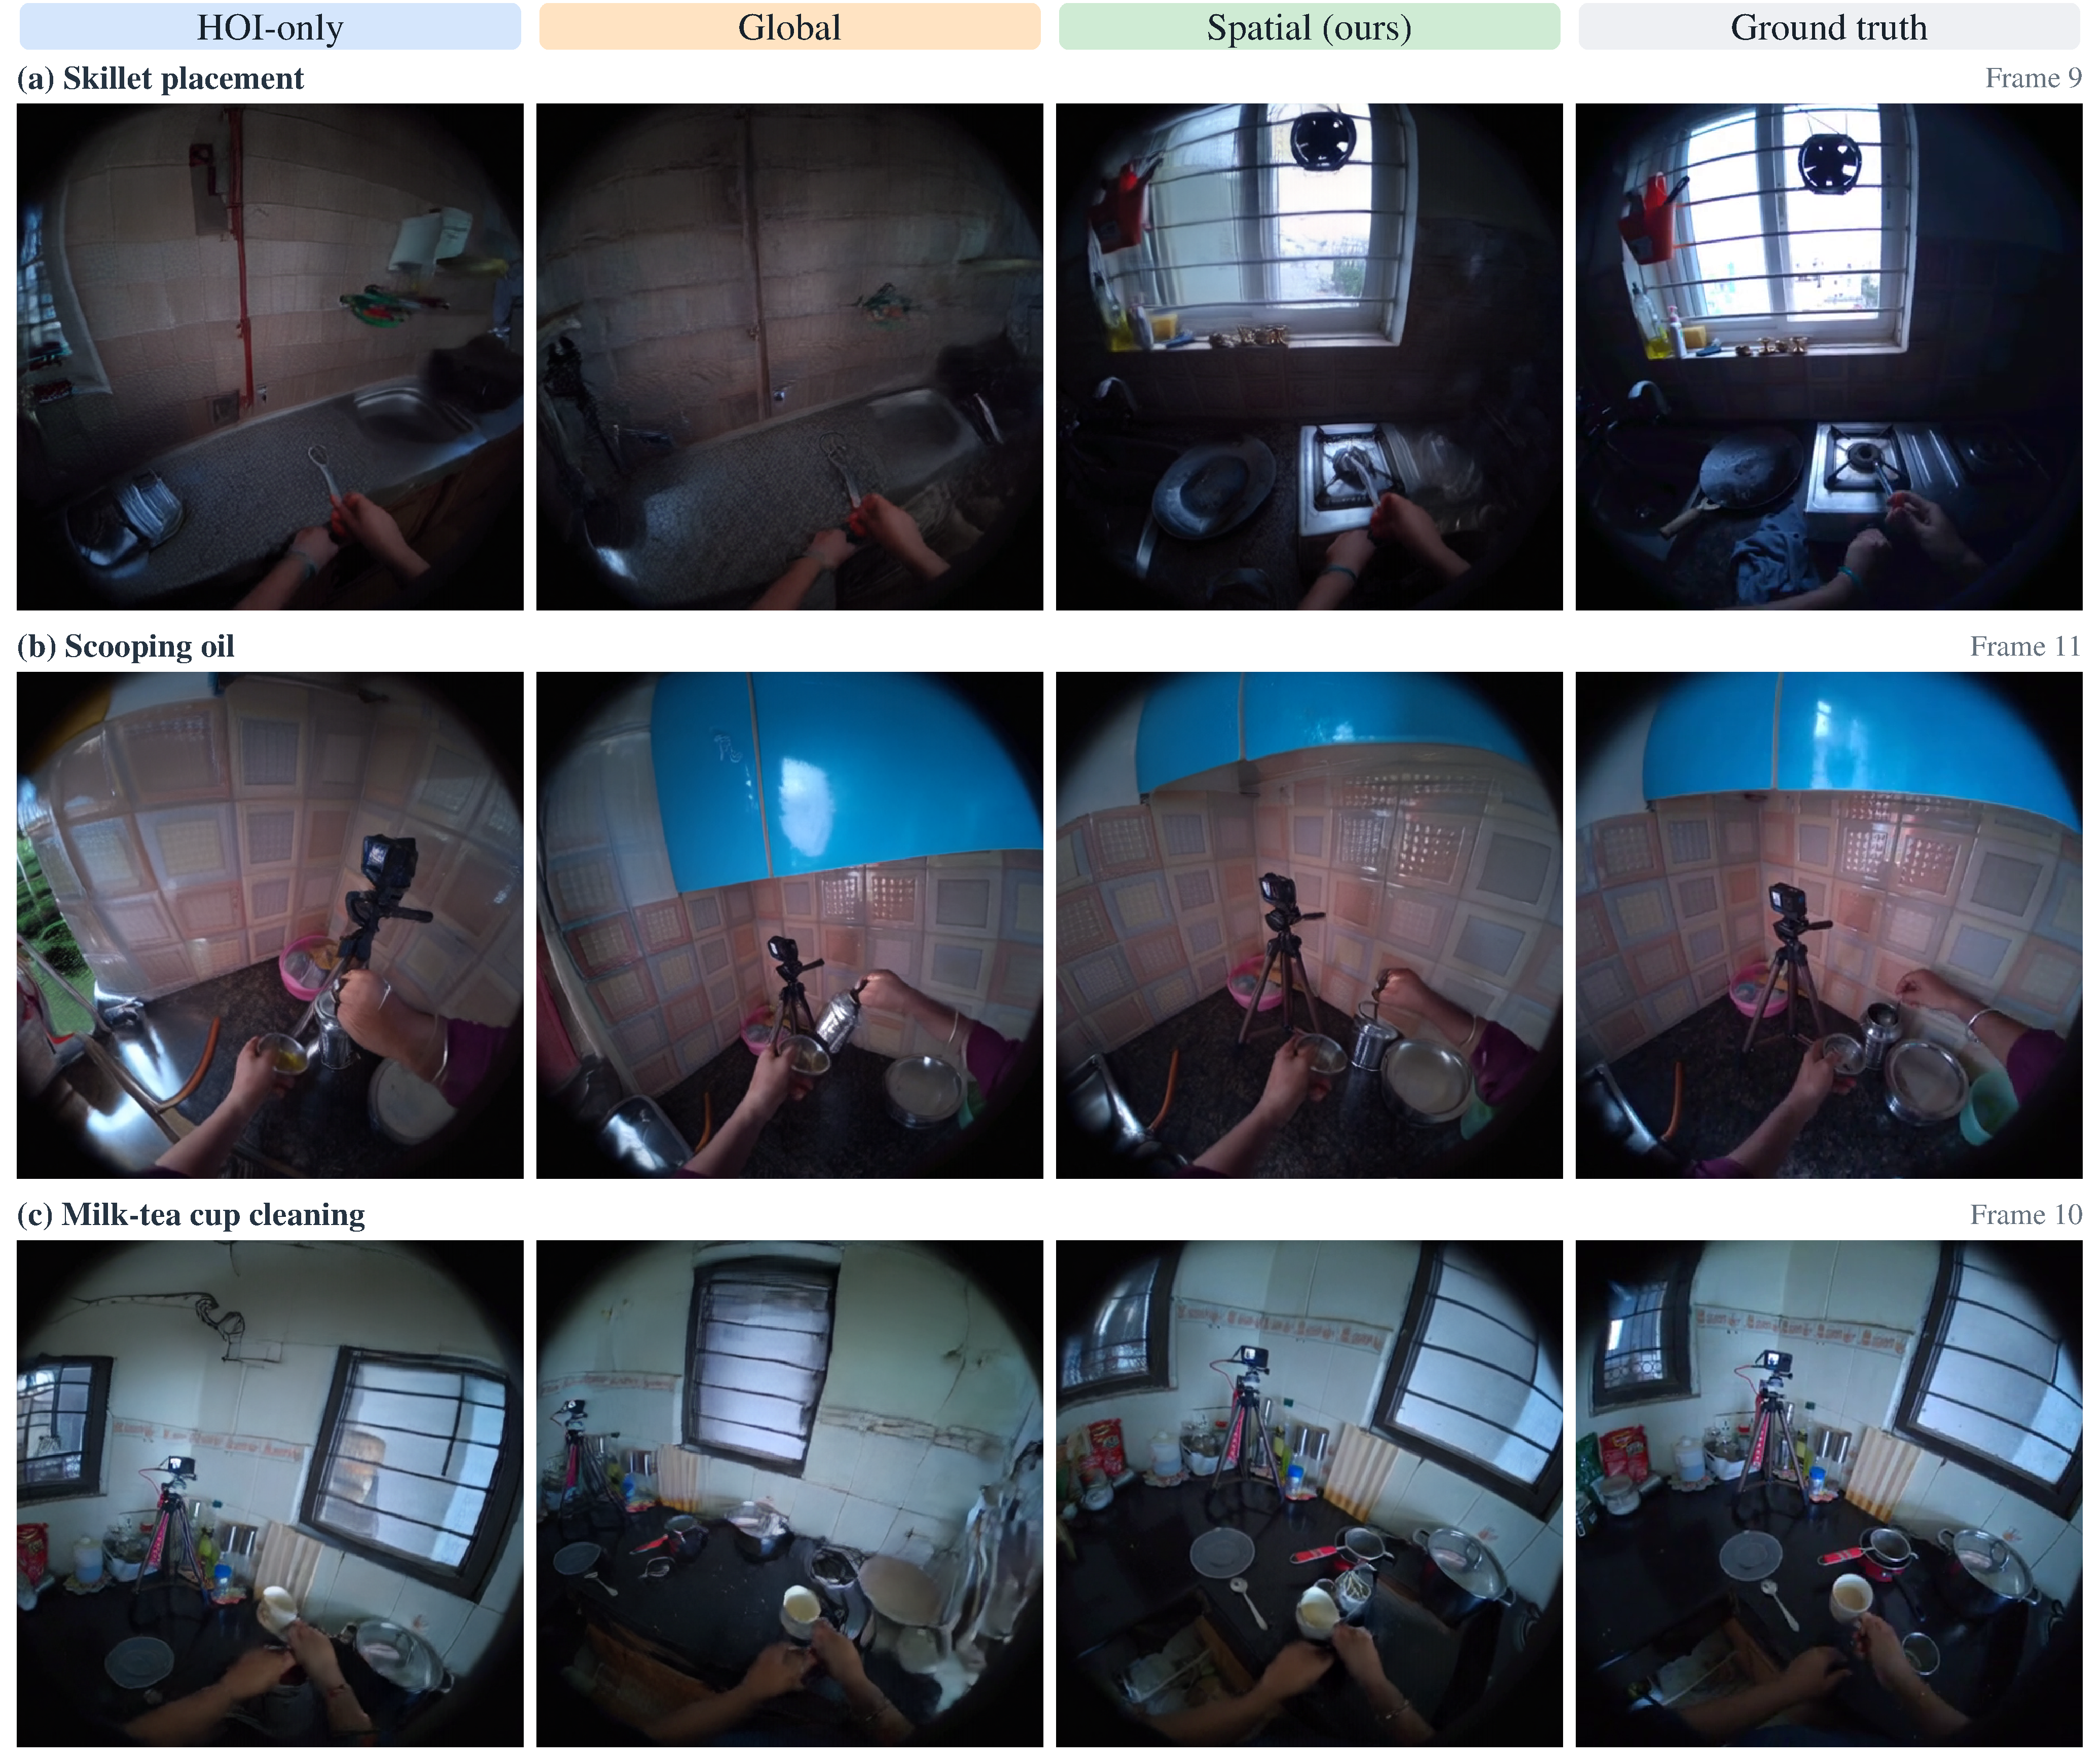
\includegraphics[width=0.52\textwidth]{figs/qual_compare/qualitative_grid.pdf}
\caption{Any2Ego preserves the viewpoint-dependent scene structure that a mask
leaves unspecified, including the layout of the cooking area in
(a) skillet placement at frame 9, the overhead cabinet in (b) scooping oil at
frame 11, and the window and background content in (c) cleaning a milk-tea cup
at frame 10. Ground truth is shown for comparison only and is never available
to any model.}
\label{fig:qual}
\end{figure}

\section{Analysis}
\label{sec:analysis}

\begin{table}[t]
\centering\small
\caption{Removing either anchor from Any2Ego costs accuracy on every metric, and
removing the textual anchor recovers EgoExo-Gen. Replacing the caption with
continuous vision-language features from a frozen Qwen3-VL-32B improves the
frame-level metrics yet leaves FVD no better than removing the anchor. Best
values are in \textbf{bold}.}
\label{tab:component}
\begin{tabular}{lC{1.5cm}C{1.5cm}C{1.5cm}C{1.5cm}}
\toprule
\textbf{Model} & \textbf{SSIM}\,$\uparrow$ & \textbf{PSNR}\,$\uparrow$ & \textbf{LPIPS}\,$\downarrow$ & \textbf{FVD}\,$\downarrow$ \\
\midrule
\textbf{Any2Ego} & \textbf{0.660} & \textbf{22.28} & \textbf{0.144} & \textbf{33.3} \\
$\;\;-$ spatial routing & 0.636 & 21.74 & 0.163 & 37.8 \\
$\;\;-$ textual anchor & 0.608 & 21.06 & 0.194 & 42.6 \\
$\;\;-$ caption, $+$ VLM features & 0.618 & 21.22 & 0.184 & 44.5 \\
\bottomrule
\end{tabular}
\end{table}

\subsection{Superiority of the Textual Anchor over Continuous Features}
\label{sec:modality}

The natural alternative to a caption is to pass continuous vision-language
features across views. To test this under a controlled comparison, we build a
continuous branch that extracts visual and instruction tokens from layer 32 of a
frozen Qwen3-VL-32B on the same 13 exocentric frames, projects the
5120-dimensional features into the video model, and injects them through a
globally gated cross-attention branch. It sits on the same frozen EgoExo-Gen base
and differs from the text branch only in what it carries.

As shown in Table~\ref{tab:component}, putting VLM features in place of the
caption improves the frame-level metrics yet leaves FVD no better than dropping
the textual anchor altogether, so it buys frame-level agreement without improving the
video distribution. Under the same gate the caption improves both, which places the
text advantage before any routing is introduced. Two properties of a caption explain
the gap. First, the converter selects interaction-relevant content over all
exocentric appearance and already states it in the target viewpoint, whereas the
continuous branch retains source-view tokens whose relation to the egocentric
scene its projection must still learn. Second, umT5 places the caption in the
space the backbone already consumes.

\subsection{Effect of Spatial Routing}
\label{sec:effect-routing}

To test the prediction of Eq.~\ref{eq:dilution} we hold everything except the
gating rule fixed, so the two variants share the frozen EgoExo-Gen base, the same
captions clip for clip, the same projections, and the same schedule.

As shown in Table~\ref{tab:component}, dropping HOI-conditioned routing back to a
global gate costs every metric without a single inversion, and the largest
margins are on FVD and LPIPS. Two features of the comparison support the dilution account. First, the route helps more on the
distributional metric than on the frame-level ones, which is expected when the
correction concentrates on a minority of tokens whose contribution to a
frame-averaged score is small. Second, the gain survives on clips where
EgoExo-Gen is already accurate, since the route can lower caption influence there
instead of paying the shared cost of a larger scalar. The results validate
routing the anchor by features the control branch has already computed, at the
cost of $30$ projection vectors of width $d$.

\subsection{Ablation Study on Anchor Content}
\label{sec:ablation}

\begin{wraptable}{r}{0.48\textwidth}
\centering\small
\caption{The trained model reads the content of both anchors, and the division of
labor is asymmetric. Win is the fraction of clips on which the original conditions
give higher SSIM than the randomized input. Best values are in \textbf{bold}.}
\label{tab:ablation}
\begin{tabular}{lC{0.95cm}C{1.0cm}C{1.0cm}}
\toprule
\textbf{Condition} & \textbf{SSIM}\,$\uparrow$ & \textbf{LPIPS}\,$\downarrow$ & \textbf{Win}\,$\uparrow$ \\
\midrule
\textbf{Original} & \textbf{0.660} & \textbf{0.144} & \\
$\;$caption rand. & 0.632 & 0.166 & 88.7\% \\
$\;$mask rand. & 0.423 & 0.504 & 100.0\% \\
\bottomrule
\end{tabular}
\end{wraptable}

A trained generator could ignore both anchors and rely on the data distribution,
so we test whether it reads their content. We keep the trained routing model fixed
and randomize one condition at a time at inference, where caption randomization
substitutes text of the same length and mask randomization moves the spatial
locations while preserving the per-class pixel budget. As reported in Table~\ref{tab:ablation}, randomizing the caption
degrades every metric and the original conditions win on $88.7\%$ of clips, while
randomizing the mask degrades them far more and wins on every clip. Both anchors are
therefore read, and they divide the work asymmetrically, as the spatial anchor
supplies the geometric skeleton while the textual anchor supplies a smaller and
consistent semantic refinement, which is what the design intends.



\begin{table}[t]
\centering\small
\caption{Residual-frame analysis after subtracting each video's own first frame
shows that Any2Ego generates real motion while image-to-video baselines mostly
retain the given frame. $\Delta$Corr is the residual correlation and $\Delta$PSNR
the residual fidelity, both higher is better, and the magnitude ratio has target
$1$. Best values are in \textbf{bold}.}
\label{tab:residual}
\begin{tabular}{lC{2.0cm}C{2.0cm}C{2.4cm}}
\toprule
\textbf{Method} & \textbf{$\Delta$Corr}\,$\uparrow$ & \textbf{$\Delta$PSNR}\,$\uparrow$ & \textbf{Mag.\ ratio}\,($\to\!1$) \\
\midrule
\textit{Ground truth} & \textit{1.000} & & \textit{1.000} \\
\midrule
Stable Video Diffusion & 0.108 & 14.85 & 1.77 \\
Wan2.2-TI2V-5B & 0.221 & 18.45 & 0.73 \\
LTX-Video & 0.233 & 18.86 & 0.61 \\
CogVideoX-5B-I2V & 0.198 & 18.76 & 0.54 \\
Wan2.1-VACE-1.3B & 0.003 & 18.09 & 0.71 \\
Wan2.1-Fun-1.3B-Control & 0.319 & 10.35 & 5.28 \\
\midrule
\textbf{Any2Ego} & \textbf{0.647} & \textbf{21.17} & \textbf{1.04} \\
$\;\;-$ spatial routing & 0.614 & 20.47 & 1.14 \\
$\;\;-$ textual anchor & 0.561 & 19.80 & 1.18 \\
\bottomrule
\end{tabular}
\end{table}

\subsection{Analysis of Residual Motion Fidelity}
\label{sec:residual}

Since the freeze-frame calibration shows that a short clip can score well by
staying still, we need a measurement that sees only what a model generates. We
subtract each video's own first frame and compare the residual fields with the
Pearson correlation ($\Delta$Corr), the residual PSNR ($\Delta$PSNR), and the ratio
of mean absolute residual magnitudes, where a model holding its first frame scores
zero correlation by construction.

As shown in Table~\ref{tab:residual}, Any2Ego reaches a residual correlation of
$0.647$ and each removed anchor lowers it in turn, while the
prompt-conditioned baselines stay near $0.20$ and reproduce only half to three
quarters of the true residual magnitude, so their frame-level scores come mostly
from retained appearance. Spatial routing also brings the magnitude ratio closest
to its target of $1$, so the textual anchor corrects the amount of motion as well
as its location. Across terciles of ground-truth motion, residual correlation
rises for spatial routing as real motion grows while it stays flat for the
baselines, which is the signature of a model copying its input frame. Overall, the residual analysis shows
that the reported gains correspond to generated motion.

\section{Conclusion}
\label{sec:conclusion}

In this paper, we introduce Any2Ego, which performs egocentric viewpoint
translation through an explicit intermediate modality anchored on text. By
separating that modality into a spatial anchor stating where an interaction
happens and a textual anchor stating what it looks like from the first person,
Any2Ego replaces one hard cross-view mapping with two easier ones, and
HOI-conditioned spatial routing applies the textual anchor where its content is
relevant. We expect the same construction wherever a cross-view mapping is too
wide to learn directly and the interaction it preserves can be stated in
language.

\section*{Reproducibility Statement}

All modules described in Section~\ref{sec:method} are implemented in the
accompanying code release, including data construction, the mask predictor,
both caption-training stages, the two generator stages, and the evaluation
pipeline. The fixed $N{=}1{,}000$ split, the freeze-frame calibration of
Eq.~\ref{eq:freeze}, and the shared frame-loading pipeline used for every
number in this paper are released with it.

\section*{Ethics Statement}

This work uses only the publicly documented Ego-Exo4D dataset of cooking
activities, which is released for research use, and we introduce no new human
data collection. The generative model studied here is scoped to short
kitchen-activity clips, and we do not evaluate or recommend it for generating
egocentric video of individuals without consent or in contexts that are
sensitive to safety, privacy, or identity.

\bibliographystyle{iclr2027_conference}
\begin{thebibliography}{99}

\bibitem[Blattmann et al.(2023)]{blattmann2023svd}
A.\ Blattmann, T.\ Dockhorn, S.\ Kulal, D.\ Mendelevitch, M.\ Kilian,
D.\ Lorenz, Y.\ Levi, Z.\ English, V.\ Voleti, A.\ Letts, V.\ Jampani, and
R.\ Rombach.
\newblock Stable Video Diffusion: Scaling Latent Video Diffusion Models to
Large Datasets.
\newblock \emph{arXiv preprint arXiv:2311.15127}, 2023.

\bibitem[Cheng et al.(2023)]{cheng2023hands23}
T.\ Cheng, D.\ Shan, A.\ Hassen, R.\ Higgins, and D.\ Fouhey.
\newblock Towards A Richer 2D Understanding of Hands at Scale.
\newblock \emph{NeurIPS}, 2023.

\bibitem[Cheng \& Schwing(2022)]{cheng2022xmem}
H.\ K.\ Cheng and A.\ G.\ Schwing.
\newblock XMem: Long-Term Video Object Segmentation with an Atkinson-Shiffrin
Memory Model.
\newblock \emph{ECCV}, 2022.

\bibitem[Grauman et al.(2024)]{grauman2024egoexo4d}
K.\ Grauman, et al.
\newblock Ego-Exo4D: Understanding Skilled Human Activity from First- and
Third-Person Views.
\newblock \emph{CVPR}, 2024.

\bibitem[HaCohen et al.(2025)]{hacohen2025ltxvideo}
Y.\ HaCohen, N.\ Chiprut, B.\ Brazowski, D.\ Shalem, D.\ Moshe, E.\ Richardson,
E.\ Levin, G.\ Shiran, N.\ Zabari, O.\ Gordon, et al.
\newblock LTX-Video: Realtime Video Latent Diffusion.
\newblock \emph{arXiv preprint arXiv:2501.00103}, 2025.

\bibitem[Jiang et al.(2025)]{vace2025}
Z.\ Jiang, Z.\ Han, C.\ Mao, J.\ Zhang, Y.\ Pan, and Y.\ Liu.
\newblock VACE: All-in-One Video Creation and Editing.
\newblock \emph{arXiv preprint arXiv:2503.07598}, 2025.

\bibitem[Kang et al.(2025)]{kang2025egox}
T.\ Kang, K.\ Kim, D.\ Kim, M.\ Park, J.\ Hyung, and J.\ Choo.
\newblock EgoX: Egocentric Video Generation from a Single Exocentric Video.
\newblock \emph{arXiv preprint arXiv:2512.08269}, 2025.

\bibitem[Liu et al.(2023)]{liu2023groundingdino}
S.\ Liu, Z.\ Zeng, T.\ Ren, F.\ Li, H.\ Zhang, J.\ Yang, C.\ Li, J.\ Yang,
H.\ Su, J.\ Zhu, and L.\ Zhang.
\newblock Grounding DINO: Marrying DINO with Grounded Pre-Training for
Open-Set Object Detection.
\newblock \emph{arXiv preprint arXiv:2303.05499}, 2023.

\bibitem[Oh et al.(2019)]{oh2019stm}
S.\ W.\ Oh, J.-Y.\ Lee, N.\ Xu, and S.\ J.\ Kim.
\newblock Video Object Segmentation using Space-Time Memory Networks.
\newblock \emph{ICCV}, 2019.

\bibitem[Peebles \& Xie(2023)]{peebles2023dit}
W.\ Peebles and S.\ Xie.
\newblock Scalable Diffusion Models with Transformers.
\newblock \emph{ICCV}, 2023.

\bibitem[Radford et al.(2021)]{radford2021clip}
A.\ Radford, J.\ W.\ Kim, C.\ Hallacy, A.\ Ramesh, G.\ Goh, S.\ Agarwal,
G.\ Sastry, A.\ Askell, P.\ Mishkin, J.\ Clark, G.\ Krueger, and I.\ Sutskever.
\newblock Learning Transferable Visual Models From Natural Language Supervision.
\newblock \emph{ICML}, 2021.

\bibitem[Ravi et al.(2024)]{ravi2024sam2}
N.\ Ravi, V.\ Gabeur, Y.-T.\ Hu, R.\ Hu, C.\ Ryali, T.\ Ma, H.\ Khedr,
R.\ R\"adle, C.\ Rolland, L.\ Gustafson, E.\ Mintun, J.\ Pan, K.\ V.\ Alwala,
N.\ Carion, C.-Y.\ Wu, R.\ Girshick, P.\ Doll\'ar, and C.\ Feichtenhofer.
\newblock SAM 2: Segment Anything in Images and Videos.
\newblock \emph{arXiv preprint arXiv:2408.00714}, 2024.

\bibitem[Ren et al.(2024)]{ren2024consisti2v}
Y.\ Ren, Y.\ Zhou, J.\ Yang, J.\ Shi, D.\ Liu, F.\ Zhang, M.\ Wang, and
X.\ Chen.
\newblock ConsistI2V: Enhancing Visual Consistency for Image-to-Video
Generation.
\newblock \emph{arXiv preprint arXiv:2402.04324}, 2024.

\bibitem[Shao et al.(2024)]{shao2024grpo}
Z.\ Shao, P.\ Wang, Q.\ Zhu, R.\ Xu, J.\ Song, M.\ Zhang, Y.\ K.\ Li, Y.\ Wu,
and D.\ Guo.
\newblock DeepSeekMath: Pushing the Limits of Mathematical Reasoning in Open
Language Models.
\newblock \emph{arXiv preprint arXiv:2402.03300}, 2024.

\bibitem[Wan et al.(2025)]{wan2025}
Team Wan, A.\ Wang, B.\ Ai, B.\ Wen, C.\ Mao, C.-W.\ Xie, D.\ Chen, F.\ Yu,
H.\ Zhao, J.\ Yang, et al.
\newblock Wan: Open and Advanced Large-Scale Video Generative Models.
\newblock \emph{arXiv preprint arXiv:2503.20314}, 2025.

\bibitem[Xu et al.(2025)]{xu2025egoexogen}
J.\ Xu, Y.\ Huang, B.\ Pei, J.\ Hou, Q.\ Li, G.\ Chen, Y.\ Zhang, R.\ Feng, and
W.\ Xie.
\newblock EgoExo-Gen: Ego-centric Video Prediction by Watching Exo-centric
Videos.
\newblock \emph{ICLR}, 2025.

\bibitem[Yang et al.(2024)]{yang2024cogvideox}
Z.\ Yang, J.\ Teng, W.\ Zheng, M.\ Ding, S.\ Huang, J.\ Xu, Y.\ Yang, W.\ Hong,
X.\ Zhang, G.\ Feng, et al.
\newblock CogVideoX: Text-to-Video Diffusion Models with An Expert
Transformer.
\newblock \emph{arXiv preprint arXiv:2408.06072}, 2024.

\end{thebibliography}

\appendix

\section{Training Configuration}
\label{app:impl}

\textbf{Mask Predictor.}\quad We train $f_{\mathrm{seg}}$ on all 108{,}338
annotated clips at $256^2$ working resolution with an ImageNet-initialized
ResNet-18 encoder, using AdamW at learning rate $5\times10^{-5}$ with
distributed data parallelism for 20 epochs. The loss follows
Eq.~\ref{eq:seg}, and we retain the ego-to-exo query curriculum of the
reference design.

\textbf{Caption Converter.}\quad To fit the six-field first-person form before
optimizing for downstream usability, difference-weighted distillation uses
32{,}562 clips and rank-16 LoRA with $\alpha=32$, under the token weights of
Eq.~\ref{eq:sft}. The reinforcement stage continues from that checkpoint with
eight candidates per input and rank-16 LoRA at learning rate $10^{-6}$, where
previews are rendered with 8 denoising steps at $256^2$ and the full setting
uses 50 steps at $480^2$. The video generator and CLIP stay frozen in both
stages.

\textbf{Generator.}\quad To separate the spatial path from the caption path,
stage one trains rank-128 LoRA on the VACE control branch under bfloat16 with gradient checkpointing. Stage two keeps the
backbone, the stage-one control LoRA, and umT5 frozen, and trains the caption
projections and gates of Eq.~\ref{eq:route}, where spatial routing adds one
token-wise projection on the detached HOI features. A single anisotropic
resize to the target square is applied identically in training, inference, and
evaluation.

\section{Evaluation Protocol}
\label{app:eval}

All methods are evaluated on the same fixed split of $N{=}1{,}000$ clips at
13 frames, where CogVideoX uses its native 30 steps and we retain the first 13 of
its 49 output frames without temporal resampling. Per-clip PSNR, SSIM, and LPIPS are
computed after resizing to $256\times256$, and FVD is pooled over the whole
split with I3D features. The exo-conditioned baselines receive raw
exocentric RGB as control input, the text-capable image-to-video baselines
receive the egocentric first frame and the task prompt, and Stable Video
Diffusion receives the first frame alone.

Coverage is counted by mapping each evaluated clip to its source take and
counting distinct take, physical-setting, task, and institution entries in the
Ego-Exo4D metadata, which yields the 281 takes, 47 settings, 13 tasks, and 10
institutions reported in Section~\ref{sec:data}. Each take contributes between
1 and 16 clips and task counts range from 3 to 240 clips, so coverage within
cooking is not uniform.

\section{Per-field Caption Results}
\label{app:caption}

\begin{table}[t]
\centering\small
\caption{Per-field caption faithfulness on the fixed 1{,}000-clip pool shows
that reinforcement improves the fields a mask leaves unspecified, with scene
and lighting gaining most. Values are mean judge scores from 1 to 5 under the
protocol of Table~\ref{tab:caption}. Best values are in \textbf{bold}.}
\label{tab:fields}
\begin{tabular}{lC{1.3cm}C{1.3cm}C{1.3cm}C{1.3cm}C{1.3cm}C{1.3cm}}
\toprule
\textbf{Caption source} & \textbf{Hands} & \textbf{Object} & \textbf{Contact} & \textbf{Scene} & \textbf{Motion} & \textbf{Lighting} \\
\midrule
\textbf{Any2Ego converter} & 4.17 & 4.18 & \textbf{4.06} & \textbf{4.70} & \textbf{3.95} & \textbf{4.63} \\
\textbf{$\;\;$w/o reinforcement} & \textbf{4.19} & \textbf{4.20} & 4.01 & 4.09 & 3.89 & 4.58 \\
\midrule
Qwen3-VL-32B & 3.09 & 3.34 & 3.20 & 4.16 & 3.14 & 4.25 \\
Qwen3-VL-235B & 2.94 & 3.38 & 3.11 & 4.15 & 3.12 & 3.89 \\
Qwen3.5-9B & 3.22 & 3.43 & 3.31 & 3.52 & 3.22 & 3.42 \\
Qwen3-VL-8B & 2.87 & 3.15 & 2.89 & 3.68 & 2.93 & 3.47 \\
\bottomrule
\end{tabular}
\end{table}

As shown in Table~\ref{tab:fields}, our converter leads on four of the six
fields, and the two stages act on different fields. Distillation establishes the
hand and object descriptions, which reinforcement leaves essentially unchanged at
$4.17$ and $4.18$. Reinforcement instead raises scene from $4.09$ to $4.70$,
which is the field whose content the HOI mask does not specify and whose
agreement with a rendered preview the reward of Eq.~\ref{eq:reward} measures.

\section{Per-clip Score Distributions}
\label{sec:dist}

Mean scores can hide a small set of clips that carries an improvement, so we
examine whether the gains hold across the pool. We compute per-clip scores
over the 13 frames of every clip in the fixed split and compare the three
Any2Ego variants under a shared kernel bandwidth. As shown in
Figure~\ref{fig:dist}, median SSIM moves from $0.613$ to $0.638$ and to
$0.657$ across EgoExo-Gen, Any2Ego without spatial routing, and Any2Ego, and median PSNR
moves from $21.27$ to
$21.80$ and to $22.35$\,dB, which tracks the means in Table~\ref{tab:main}
and indicates that the improvement is not driven by a tail. The distribution
of spatial routing is close to symmetric, with a 10th to 90th percentile
interval of $[0.566,0.760]$ for SSIM and $[19.02,25.22]$\,dB for PSNR.
Overall, the per-clip distributions show that the textual anchor shifts the
whole pool instead of a favorable subset.

\begin{figure}[t]
\centering
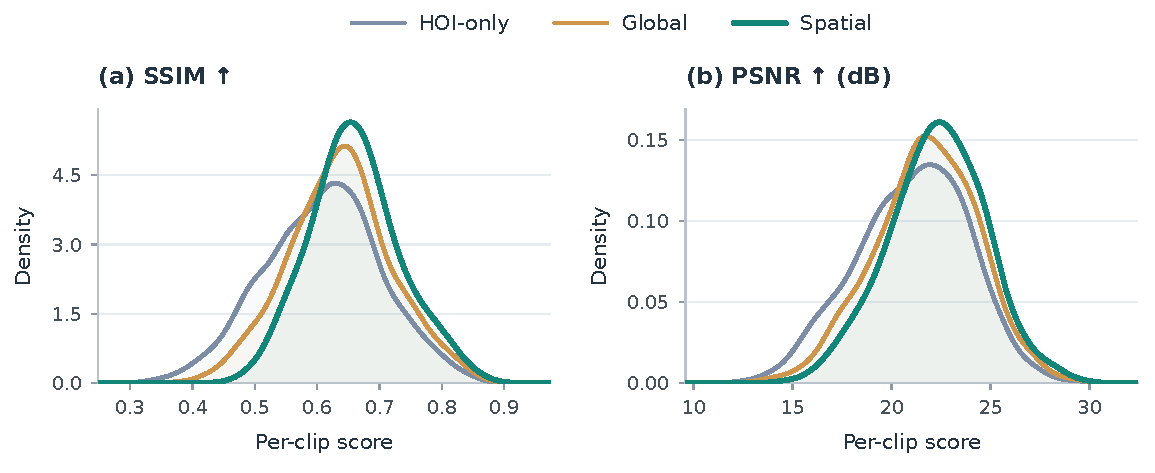
\includegraphics[width=\textwidth]{figs/metric_distributions_ssim_psnr.pdf}
\caption{The textual anchor shifts the whole evaluation pool instead of a
favorable subset, since per-clip (a) SSIM and (b) PSNR distributions move
together across EgoExo-Gen, Any2Ego without spatial routing, and Any2Ego under a shared
kernel bandwidth.}
\label{fig:dist}
\end{figure}

\section{Additional Qualitative Examples}
\label{app:qual}

\begin{figure}[t]
\centering
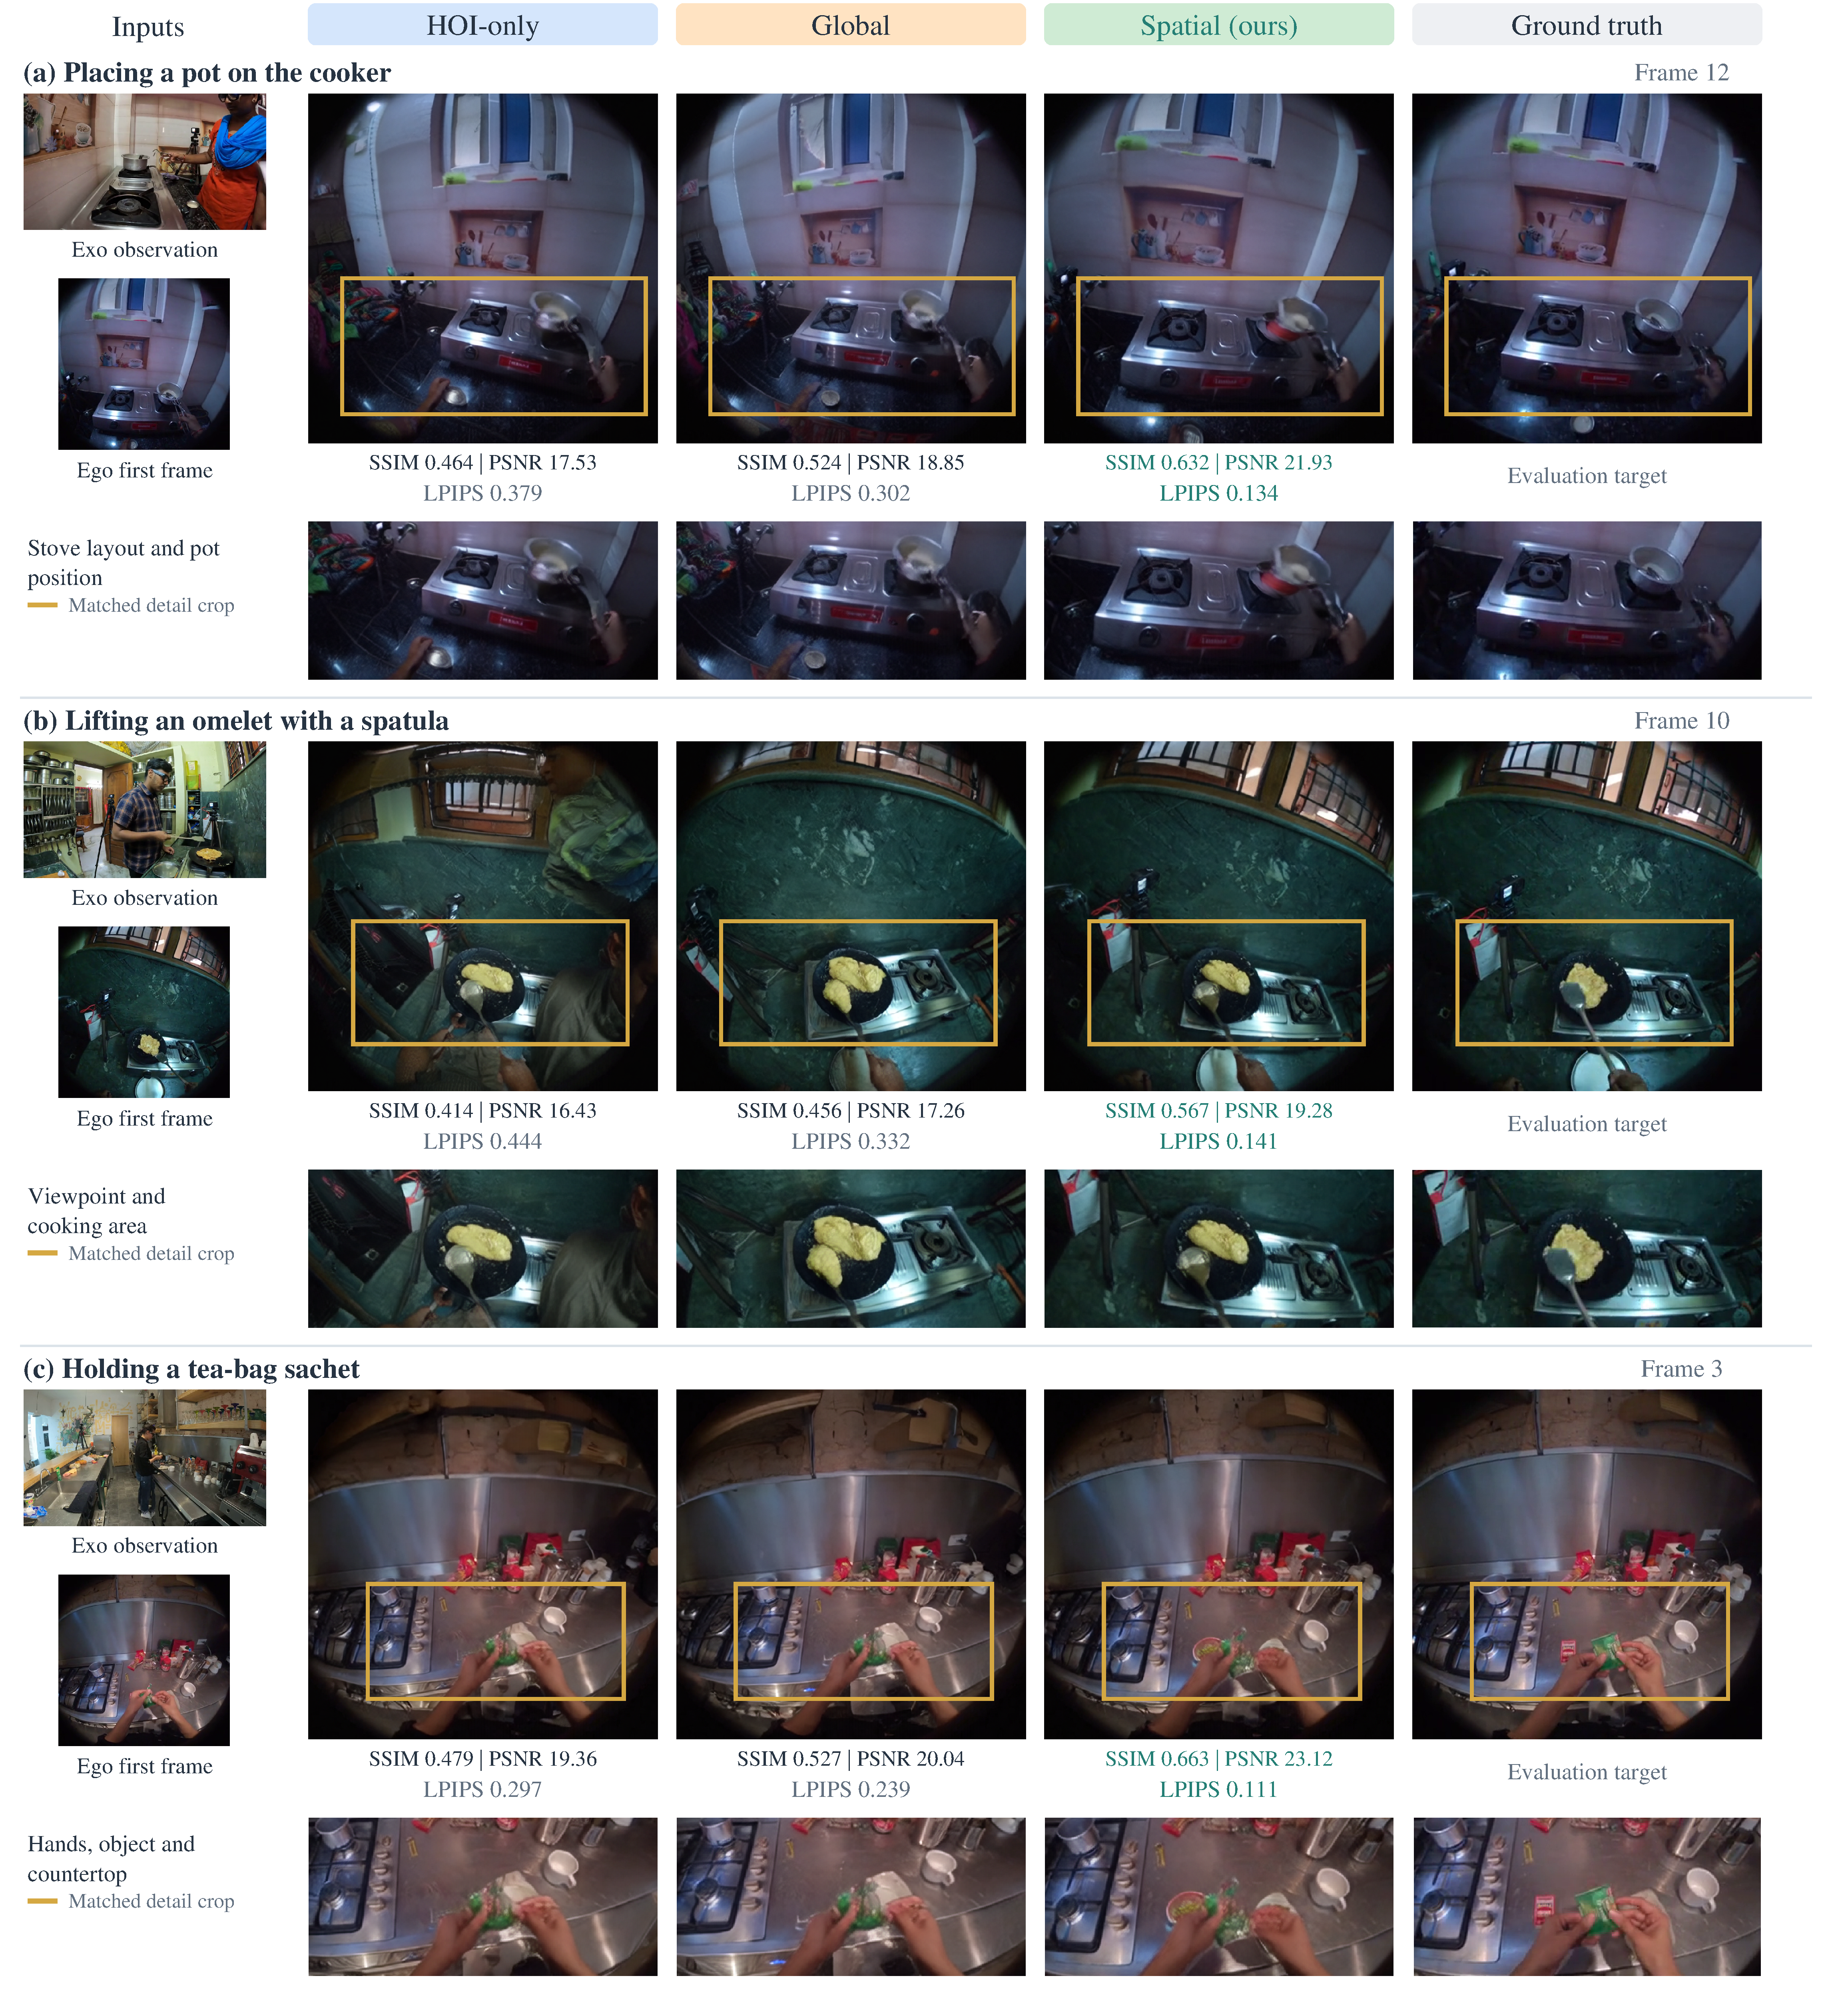
\includegraphics[width=\textwidth]{figs/appendix_cases.pdf}
\caption{Spatial routing follows the ground-truth framing of the cooking area
more closely on three further cases, including (a) placing a pot on the cooker
at frame 12, (b) lifting an omelet with a spatula at frame 10, and (c) holding
a tea-bag sachet at frame 3. Gold boxes mark identical crop coordinates across
methods, and the reported scores are computed over the full 13-frame clip.}
\label{fig:appendix-cases}
\end{figure}

As shown in Figure~\ref{fig:appendix-cases}, the pot-placement and omelet
cases differ mainly in stove layout and viewpoint, where spatial routing
follows the ground-truth framing of the cooking area more closely, and the
tea-bag case gives a closer view of the hands, the handled object, and the
countertop. Each row compares the same time step across methods with matched
crops, and frame indices start at $0$.

\end{document}
